% В этом шаблоне используется класс spbau-diploma. Его можно найти и, если требуется, 
% поправить в файле spbau-diploma.cls
\documentclass{spbau-diploma}
\usepackage{graphicx}
\usepackage{amsmath}
\usepackage{subcaption}
\begin{document}
% Год, город, название университета и факультета предопределены,
% но можно и поменять.
% Если англоязычная титульная страница не нужна, то ее можно просто удалить.
\filltitle{ru}{
    chair              = {\ },
    title              = {\textbf{ВЫПУСКНАЯ КВАЛИФИКАЦИОННАЯ РАБОТА\\(БАКАЛАВРСКАЯ РАБОТА)}\vskip 0.5 em на тему \vskip 0.5 em\textbf{«Методы оценки сложности текстовых данных для ускорения обучения языковых моделей с помощью обучения по плану»}\\\textit{\small Направление подготовки 01.03.02 Прикладная математика и информатика}},
    % Здесь указывается тип работы. Возможные значения:
    %   coursework - Курсовая работа
    %   diploma - Диплом специалиста
    %   master - Диплом магистра
    %   bachelor - Диплом бакалавра
    % type               = {diploma},
    position           = {студента},
    group              = {БПМ171С},
    author             = {Сурков Максим Константинович},
    supervisorPosition = {?},
    supervisor         = {Ямщиков Иван Павлович},
    reviewerPosition   = {ст. преп.},
    reviewer           = {Привалов А.\,И.},
    % chairHeadPosition  = {д.\,ф.-м.\,н., профессор},
    % chairHead          = {Омельченко А.\,В.},
    university = {\textbf{Федеральное государственное автономное образовательное учреждение высшего образования\\«Национальный исследовательский университет\\«Высшая школа экономики»}},
    faculty = {Факультет Санкт-Петербургская школа физико-математических и компьютерных наук\\Департамент информатики},
    city = {Санкт-Петербург},
    year = {2021}
}
\maketitle

\tableofcontents
\section*{Аннотация}
\ 

Современные системы обработки естественного языка активно используют глубокие нейронные сети (BERT, GPT-3), которые требуют значительных ресурсов для их обучения. За последние годы было разработано множество подходов для решения данной проблемы. Одним из них является обучение по плану. Данный метод состоит из двух составляющих: оценки сложности тренировочных данных и алгоритма их семплирования. Основной целью данной работы является исследование метрик оценки сложности текстовых данных в контексте обучения по плану и влияния данного метода ускорения обучения на скорость сходимости языковых моделей на задачах предобучения и классификации. В процессе исследований было предложено и адаптировано несколько подходов из разных областей математики. Также были реализованы производительные алгоритмы вычисления найденных метрик на больших объемах данных в несколько десятков миллинов тренировочных примеров. Объемный набор экспериментов на задачах предобучения и классификации  выявил наиболее эффективные метрики для использования в обучении по плану. В то же время было установлено, что обучение по плану негативно влияет на скорость сходимости на задаче предобучения, однако не уступает базовому подходу (обучению без плана) на задаче классификации. Также был рассмотрен важный частный случай обучения языковой модели на шумном наборе тренировочных данных. Сравнительный анализ показал ускорение обучения до двух раз для достижения 95\% итоговой точности модели при применении обучения по плану с наиболее эффективной метрикой.
\\

Ключевые слова: обработка естественного языка, обучение по плану, теория информации, оценка сложности текстовых данных

\pagebreak

Modern state-of-the-art natural language processing systems use deep neural networks (BERT, GPT-3) that require many resources for training. Several techniques have been developed for the last ten years. One of them is curriculum learning, which consists of two parts, namely data complexity evaluation and sampling. The main purpose of this work is to research metrics of text complexity in the context of curriculum learning and explore the influence of curriculum learning on training time on pre-training and classification tasks. Several approaches from different mathematics fields were suggested and adapted during the research. Moreover, efficient algorithms for calculating given metrics on large datasets of several tens of millions of samples were implemented. Extensive experiments highlighted the most efficient metrics for use in curriculum learning. At the same time, it was established that curriculum learning negatively affects convergence time on pre-training task, but not inferior to the basic solution (learning without curriculum) on the classification task. Also, training on a noisy training dataset was considered. Comparative analysis showed a double reduction in training time needed to achieve 95\% of final model accuracy using curriculum learning with the most effective metric.

Keywords: natural language processing, curriculum learning, information theory, text complexity estimation
\section*{Введение}
\ 

На сегодняшний день существует множество сфер, где активно применяется обработка естественного языка. Например, в разработке голосовых помощников, алгоритмов фильтрации текста и машинного перевода. Возникающие задачи необходимо решать эффективно с точки зрения качества модели и скорости работы системы. За основу многих подходов взят механизм внимания~\cite{vaswani2017attention}. На его базе были разработаны модели, такие как BERT~\cite{devlin2018bert}, GPT-3~\cite{brown2020language} и многие другие. Данные сети имеют высокое качество, однако, за это приходится платить существенным временем обучения. В рамках данной работы исследуется влияние обучения по плану на примере тренировки модели BERT, так как она является одной из самых популярных моделей, имеет высокую точность и сравнительно небольшой размер для удобства постановки экспериментов. Также стоит отметить, что для обучения модели используют объемные корпуса данных, состоящие из нескольких десятков миллионов примеров, для которых нужны производительные алгоритмы их обработки. 

\begin{table}[h]
	\caption{Количество примеров в тренировочных корпусах данных}
	\label{table:dataset_sizes}
	\centering
	\begin{tabular}{|l|c|}
		\hline
		Корпус данных & Размер \\
		\hline\hline
		Wikipedia & 3-600M \\
		BooksCorpus & 74M\\
		\hline\hline
		Hyperpartisan News Detection & 600k-2M \\
		sentiment140 & 1.6M \\
		IWSLT & 200-230k \\
		QQP & 364k \\
		MNLI & 393k \\
		\hline
	\end{tabular}
\end{table}

Процесс тренировки модели состоит из двух основных частей. Первая заключается в предобучении сети на задаче Masked Language Modelling~\cite{devlin2018bert}, которая состоит в восстановлении предложения после замены 15\% случайных слов на пробелы. Предобучение занимает несколько недель исполнения кода на дорогостоящих графических процессорах. Второй этап представляет из себя задачу дообучения языковой модели, например на задачу классификации, и требует несколько дней даже на элементарных задачах, таких как определение спама или грубой речи~\cite{gertner2019mitre}. Одним из методов ускорения обучения моделей является обучение по плану~\cite{bengio2009curriculum}. При его применении данные сортируются по сложности, а затем семплируются с помощью заранее определенного алгоритма, который учитывает порядок данных. Отмечю, что в рамках данной работы исследуются метрики оценки сложности текстов, а семплеры рассматриваются из уже существующих работ. Обучение по плану хорошо себя показало во многих областях машинного обучения~\cite{narvekar2020curriculum, hacohen2019power, mermer2017scalable}. Однако, в последнее время стали появляться работы с отрицательными результатами применения обучения по плану, что показывает спорную репутацию данного подхода к ускорению. Например, в работе~\cite{wu2020curricula} показано ухудшение качества итоговой модели и замедление ее обучения на задачах классификации картинок при использовании обучения по плану. В то же время, в тех же статьях авторы находят частные случаи применения обучения по плану на практике, одним из которых является обучение на шумных тренировочных данных. К сожалению, на данный момент существует ограниченное число работ, исследующих вопрос применения обучения по плану в обработке естесственного языка. Важно отметить, что нет работ, где обучение по плану применяется на задачах предобучения языковых моделей и классификации текстов. Более того, авторы уделяют большое внимание алгоритмам семплирования данных, а метрики берут из достаточного узкого множества, которое можно значительно расширить, применив различные сферы компьютерных наук. Также, во многих статьях основной целью является улучшение качества итоговой модели, а скорость обучения уходит на второй план. Наконец, нет работ, освещающих важный частный случай обучения моделей на шумных тренировочных данных. Таким образом, основная исследовательская мотивация заключается в изучении вопроса применимости обучения по плану на задачах предобучения языковых моделей и классификации текстов при использовании больших моделей, таких как BERT, и нахождении метрик оценки сложности текстов, которые можно использовать в контексте обучния по плану.

\subsection*{Цель и задачи}
\ 

Целью данной работы является исследование возможности ускорения обучения языковой модели BERT на задачах предобучения языковых моделей и классификации текстов c помощью обучения по плану за счет применения улучшенной метрики сложности текстовых данных

\vspace*{20pt}
Задачи:
\begin{itemize}
	\item Предложить метрики оценки сложности текста
	\item Реализовать производительные алгоритмы вычисления предложенных метрик на больших корпусах данных
	\item Исследовать влияние найденных метрик на скорость обучения языковой модели BERT на чистых и шумных тренировочных данных
\end{itemize}
\pagebreak
\subsection*{Достигнутые результаты}
\ 

В рамках данной работы был предложен ряд метрик оценки сложности текстовых данных, расширяющий множество уже существующих подходов: TF-IDF, EE, TSE, TPW, MlM-loss, а также производительные алгоритмы для их вычисления на больших объемах данных. Было произведено объемное исследование влияния обучения по плану на задачах предобучения и классификации при использовании чистых тренировочных данных, в результате которого было выяснено, что:

\begin{itemize}
	\item Обучение по плану замедляет обучение на задаче предобучения от 2 до 5 раз
	\item Общая тенденция заключается в том, что обучение по плану не ускоряет обучение на задаче классификации, однако существует узкий набор конфигураций, который позволяет сократить число тренировочных шагов на 3\% в среднем
\end{itemize}

Наконец, был рассмотрен важный частный случай обучения языковых моделей на шумных тренировочных данных. В результате изучения была выявлена метрика TPW (среднее число токенов на слово), которая позволяет обучить модель до 95\% итоговой точности в два раза быстрее по сравнению с обучением без плана.

\subsection*{Структура работы}
\ 

\begin{itemize}
	\item В главе \ref{sec:literature} рассматриваются релевантные работы в области обработки естественного языка и обучения по плану
	\item В главе \ref{sec:metrics} предлагаются метрики оценки сложности текстов вместе с производительными алгоритмами для их вычисления на больших объемах данных
	\item В главе \ref{sec:experiments} описываются эксперименты, проведенные в рамках данной работы, анализируются результаты на задачах предобучения и классификации, а также рассматривается частный случай обучения языковых моделей на шумных тренировочных данных
	\item В последней главе делаются выводы по результатам всей работы, а также предлагаются направления для дальнейших исследований
\end{itemize}

\section{Обзор литературы} \label{sec:literature}
\subsection{Современные подходы к решению задач обработки естественного языка}
\ 

Несколько лет назад большинство подходов к решению задач обработки естественного языка так или иначе включали в себя использование рекуррентных или сверточных нейронных сетей в сочетании с механизмом внимания. Это накладывало некоторые ограничения на производительность моделей, так как данные методы тяжело распараллелить, что приводит к большому потреблению времени. В 2017 году Vaswani со своими коллегами в их работе~\cite{vaswani2017attention} описали изобретенную ими новую архитектуру глубокой нейронной сети под названием трансформер. Данная модель полностью основана на механизме внимния и не включает в себя рекуррентные или сверточные нейронные сети. Вместо этого авторы используют так называемый multi-head attention слой. Это позволяет производить обучение в параллельном режиме. Используя это свйоство, ученые добились многократного ускорения обучения модели при увеличении качества модели на несколько BLEU пунктов на задачах машинного перевода.

Спустя некоторое время после этого прорыва компания Google выпустила работу, посвященную модели BERT~\cite{devlin2018bert} (Bidirectional Encoder Representations from Transformers). Авторы придумали способ предобучения трансформеров, который бы позволил модели учитывать как префиксный контекст, так и суфиксный во время совершения предсказания. Это свойство очень важно при решениии целого класса задач. Например, при ответе на вопрос важно, чтобы модель обрабатывала конкретную часть предложения, понимая, что происходит до и после данной части. Их метод предобучения заключается в решении двух следующих задач. Первая задача называется MLM (Masked Language Modelling) и заключается в восстановлении предложения после скрытия некоторой его части (авторы скрывают 15\% текста). Во второй задаче под названием NSP (Next Sentence Prediction) нужно по двум предложениям понять, правда ли, что второе предложение является продолжением первого. В результате это привело к улучшению качества итоговой модели на целом ряде задач, связанных с ответами на вопросы, классификацией текстов и нахождением именованных сущностей в тексе, на несколько процентов по сравнению с лучшими моделями того времени. 

Стоит отметить, что после появления данной статьи стало появляться множество модификаций и аналогов модели BERT~\cite{lan2019albert,lewis2019bart,he2020deberta,sanh2019distilbert,le2019flaubert,nguyen2020phobert,liu2019roberta,iandola2020squeezebert}. Это говорит о большом потенциале трансформеров и методов их предобучения, а также о наличии широкого ряда свойств, позволяющих улучшать качество решений задач в машинном обучении.

Также существует альтернативный подход к решению задач обработки естественного языка, опирающийся на другую философию. В 2020 году Brown и др. представили в своей работе~\cite{brown2020language} новую модель под названием GPT-3. Она имеет в 1000 раз больше весов и способна научиться решать конкретную задачу, увидев всего несколько примеров. Это говорит о том, что данный метод позволяет получить очень устойчивую модель, которая не будет переобучаться на распределение датасета конкретной задачи.

Видно, что существует широкое множество разных задач, к каждой из которых нужен свой подход. Однако, в 2020 году в той же компании Google был предложен подход, унифицирующий широкий ряд задач и сводящий каждую из них к задаче в формате "text-to-text". Данный фреймворк и модель, предложенную авторами называют T5 (Text-to-Text Transfer Transformer). Авторы добились с помощью этого универсального метода резульататов, сравнимых с лучшими моделями на момент выхода их работы.

\subsection{Альтернативные способы ускорения обучения языковых моделей}
\ 

Большинство современных подходов к решению задач обработки естественного языка используют большие нейронные сети, состоящие из нескольких сотен миллионов параметров. Данные модели требуют большого количества времени как для обучения, так и для их использования. Поэтому люди всячески стараются побороть эту проблему. Помимо обучения по плану, которое явяется объектом изучения данной работы, существует множество алтернативных подходов к оптимизации языковых моделей.

В машинном обуении есть подход к уменьшению размера сети, который называется дистилляцией знаний (knowledge distillation). Суть его заключается в том, что большая сеть рассматрвиается как учитель. В качестве студента строят модель, имеющую схожую архитектуру, но содержащую на порядок меньше параметров. Затем модель-студента обучают, используя специальную функцию потерь. Данный подход был успешно прменен к дистилляции модели BERT в работе~\cite{sanh2019distilbert}, где авторы построили модель под названием DistilBERT. Ученые использовали линейную комбинацию трех функций потерь: $L_{mlm}$ (фукнция потерь от задачи Masked Language Modelling), $L_{ce}$ (функция потерь дистилляции) и $L_{cos}$ (функция потерь, минимизирующая косинусное расстояние между скрытыми состояниями модели-учителя и модели-студента). Авторы добились уменьшения размера модели на 40\%, ускорения использования на 60\%, сохранив 97\% качества модели-учителя.

Существует подход, который позволяет сократить размер сети, не меняя архитектуру модели. Этот метод называется квантизацией. Он нашел удачное применение и в обработке естественного языка в работе~\cite{shen2020q}, где авторы представили новую модель Q-BERT. Методология заключается в том, чтобы трансформировать вещественнозначные числа с плавающей точкой в дискретное множество чисел, которое будет задаваться множеством отрезков. Тогда каждому вещественному числу будет соответствовать некоторый отрезок, в который данное число попало. Ученые заметили, что две самые большие части модели BERT -- это энкодер и эмбеддинги, поэтому они добавили квантизацию только в эти части. Также было выявляно, что разные части модели нужно квантизировать по-разному. Это связано с тем, что некоторые слои более чувствительны к каким-либо изменениям, в то время как другие позволяют применять более агрессивную квантизацию. Ученые определяют степень квантизации, используя специальную метрику, основанную на подчете среднего модуля самых больших собственных чисел матрицы Гессе второго порядка, а также на подсчете среднего отклонения данной величины. Таким образом, чем больше модуль самого большого собственного числа, тем более чувствителен слой к применению квантизации. Наконец, авторы вводят так называемую групповую квантизацию, разделяя слои на несколько групп, в каждой из которых применяется отдельная квантизация. Описанные в данной работе методы позволили сократить вес модели в несколько раз, потеряв при этом всего 2.3\% точности.

Еще одним способом оптимизации моделей является так называемый прунинг (pruning). Метод заключается в удалении некоторого подмножеста весов нейронной сети так, чтобы модель сохраняла итоговое качество. Данный подход применили в работе~\cite{gordon2020compressing}. Авторы исследовали влияние прунинга на качество модели BERT, используя три разных режима: низкий (30-40\%), средний и высокий уровень прунинга. Для того, чтобы применить прунинг уровня $\alpha$, нужно найти средние магнитуды весов сети и вырезать $\alpha$ весов с самой маленькой магнитудой. Выяснилось, что низкий уровень прунинга позволяет сократить размер модели в несколько раз с сохранением итогового качества. Однако, при увеличении уровня прунинга модель начинает деградировать.

Для того, чтобы ускорить обучение языковой модели, можно оптимизировать различные объекты, которые так или иначе учавствуют в этом процессе. Выше были рассмотрены методы, вторгающиеся во внутреннюю структуру модели. Обучение по плану же использует ускоряемую нейронную сеть как черный ящик. Аналогичным образом поступает так называемый метод оптимизации большого батча (large batch optimization). Одним из первых наиболее удачных применений данной техники является алгоритм Lars~\cite{you2017scaling}. Однако, он плохо обобщается до моделей, использующих механизм внимания. Эту проблему решили You и др. в работе~\cite{you2019large}, предложив модификацию способа послойной адаптации скосрости обучения (learning rate), который авторы назвали Lamb. Новый алгоритм позволяет увеличивать размера батча до 30k+ примеров (без потери итогового качества), что приводит к возможности предобучить BERT за 76 минут.

lotery ticket hypo
	
\subsection{Возникновение обучения по плану}
\ 

Точная дата возникновения обучения по плану не известна, но можно выделить логическое начало в работе Bengio 2009 года~\cite{bengio2009curriculum}, в которой было показано, что обучение по плану может привести к улучшению качества моделей машинного обучения. Авторы поставили несколько экспериментов, одним из которых является опыт по обучению классификатора геометрических фигур. Было обнаружено, что если сначала предъявить модели более простые примеры (квадраты, круги, равнобедренные треугольники) перед стандартным алгоритмом обучения, то итоговое качество возрастет. Этот простой пример подчеркивает большой потенциал обучения по плану к улучшению существующих алгоритмов в машинном обучении.
\subsection{Применение обучения по плану в смежных сферах машинного обучения}
\ 

Обучение по плану активно применялось в разных областях машинного обучения в течение последних нескольких лет. Например, Hacohen и Weinshall в 2019 году~\cite{hacohen2019power} применили данный метод к задачам компьютерного зрения. Они предложили модельную метрику оценки сложности картинок, которая считается следующим образом. Рассматривается независимая модель, предобученная на датасете ImageNet. Далее сложность примера определяется как уверенность модели в своем предсказании. Наконец, ученые использовали лестничный алгоритм семплирования в паре с предложенной метрикой. В результате был получен прирост в скорости обучения и в качестве итоговой модели.

Обучение по плану применяется и в классическом глубоком обучении. Mermer и др.~\cite{mermer2017scalable} предложили способ автоматической оценки сложности векторных данных для решения задачи классификации. Для этого авторы для каждого примера строят распределение вероятностей классов двумя способами.
\begin{enumerate}
	\item на базе $k$ ближайших соседей. Рассмотрим мультимножество меток соседей, тогда вероятность $i$-го класса равна доле соседей с данной меткой
	\item на базе ансамбля. Обучим $k$ независимых классификаторов стандартным алгоритмом. Далее для каждой метки определим среднюю предсказанную классификаторами вероятность того, что данный пример имеет рассматриваемую метку
\end{enumerate}
	
В итоге сложность примера вычисляется как энтропия построенного распределения. Авторы рассмотрели $36$ датасетов, на многих из которых обучение по плану выиграло у стандартного алгоритма обучения. Заметим, что подход, основанный на метках соседей, невозможно применить к текстам в явном виде, так как примеры из естественного языка не имеют векторной структуры. Однако можно рассмотреть пространство эмбеддингов. Но данный способ будет зависеть от метода получения векторного представления текстов. Более того, размеры датасетов обучения языковых моделей состоят из большого числа примеров, и поиск $k$ ближайших соседей может требовать большого количества времени, что недопустимо при решении задачи ускорения обучения. Те же самые проблемы возникают и при применения подхода, основанного на ансамблировании.

Важно отметить, что при применении обучения по плану можно получить и отрицательный результат. Так Wu и др.~\cite{wu2020curricula} выявили негативное влияние обучения по плану на скорость обучения широкого множества глубоких нейронный сетей на задаче классификации картинок. Авторы применили данный подход к более чем сотне архитектур, среди которых ResNet и VGG-19. Авторы рассмотрели несколько метрик сложности данных, которые сильно коррелировали с величиной $s(x_i, y_i)$ последней эпохи $t$	, после которой модель $w$ правильно отвечает на пример $(x_i, y_i)$ вплоть до последней эпохи $T$ (предсказание модели $\hat{y}_w(t)$ совпадает с реальной меткой $y_i$ примера), для которого считается сложность (формула~(\ref{eq:learned_epoch})). 

\begin{equation} \label{eq:learned_epoch}
s(x_i, y_i) = \min_{t^*}\{\hat{y}_w(t)_i = y_i,\forall t^* \le t \le T\}
\end{equation}

Было использовано семейство "префиксных" семплеров (рис.~\ref{fig:cv_pacing_functions}), а именно возрастающих функций, которые определяют долю легких примеров $g(t)$ в конкретный момент обучения $t$. Таким образом, данные семлперы в момент времени $t$ строят батч данных, равноверятно выбирая примеры из первых $g(t)$ семплов отсортированного по метрике сложности датасета. В результате, ученые показали, что использование данной конфигурации обучения по плану не приводит ни к улучшению качества итоговой модели, ни к ускорению обучения. Также было рассмотрено два важных частных случая, а именно обучение на шумных данных и обучение с ограниченным числом тренировочных шагов. При добавлении 20\% шума в тренировочный корпус, обучение по плану позволяет улучшить точность модели на 10\%. Влияние же подхода на скорость обучения исследовано не было.

\begin{figure}[h]
	\centering
	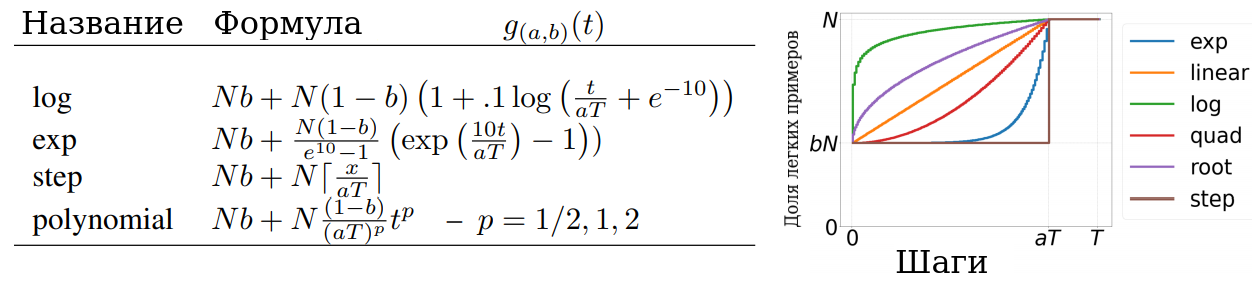
\includegraphics[scale=0.48]{CV_pacing_functions}
	\caption{Семейство функций для семплирования данных}
	\label{fig:cv_pacing_functions}
\end{figure}

\subsection{Применение обучения по плану в обработке естественного языка}
\ 

В обработке естественного языка существует ограниченное число существенных результатов в контексте применения обучения по плану. Вероятно, это связано с тем, что естественный язык состоит из слов и предложений, не имеющих строгую структуру, которую сложно формально описать. Более того, на данный момент наука не понимает всех процессов, происходящих внутри современных языковых моделей.

Platanios и др.~\cite{platanios2019competence} исследовали влияние обучения по плану на задаче машинного перевода на скорость сходимости нейронных сетей. Авторы рассмотрели две метрики сложности текстов: длину и вероятность правдоподобия, которая вычисляется по формуле (\ref{eq:log_likelihood}), где $s_i$ -- текст или набор токенов, $w_k^i$ -- слово или токен, $p(x)$ -- доля токенов $x$ во всем датасете.

\begin{equation} \label{eq:log_likelihood}
d(s_i) = -\sum\limits_{k=1}^{N}\log p(w_k^i)
\end{equation}

Они показали, что правдоподобие не имеет никаких преимуществ по сравнению  с длиной с точки зрения скорости обучения моделей. В качестве семплеров был взят префиксный семплер с функцией $c(t)$ (формула (\ref{eq:competence_based_sampler})), вычисляющий долю простых примеров, доступных для построения батча.

\begin{equation} \label{eq:competence_based_sampler}
c(t) = \min\left(1, \sqrt{t\frac{1 - c_0^2}{T} + c_0^2}\right)
\end{equation}

$T$ -- общее число тренировочных шагов, $c_0$ -- доля простых примеров, доступных в самом начале обучения (авторы используют $c_0 = 0.01$)

В итоге, ученые добились улучшения качества модели на 2.2 BLEU и ускорения обучения на 70\%.

Xu и др.~\cite{xu2020curriculum} предложили альтернативный способ применения обучения по плану в обработке естественного языка на задаче Natural Language Understanding. Их метод оперирует понятием модельной оценки сложности текстов. Сложность примеров меняется в процессе обучения в зависимости от качества модели на момент применения метрики к примеру. Авторы предлагают алгоритм, который в цикле повторяет следующую процедуру. Тренировочный корпус данных разделяется на несколько частей. Затем, для каждого блока независимо обучается новая модель, которая инициализируется весами текущей глобальной модели. После этого оценивается сложность всех примеров как сумма уверенностей всех моделей по всем блокам кроме блока, в котором находится данный пример (рис. \ref{fig:acl20_algo_difficulty}).

\begin{figure}[h]
	\centering
	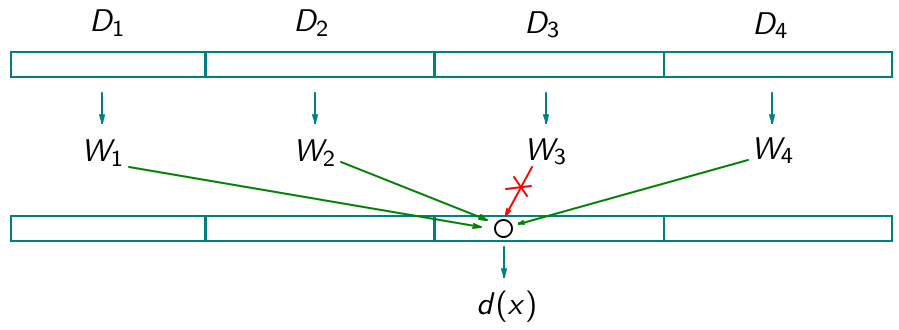
\includegraphics[scale=0.48]{acl20_algo_difficulty}
	\caption{Алгоритм вычисления модельной метрики сложности текста. На данной схеме датасет делится на $4$ части, на каждой из которых учится независимая модель BERT с началными весами текущей глобальной модели. Сложность примеров в блоке под номером $3$ вычисляется как сумма уверенностей моделей $W_1,W_2,W_4$.}
	\label{fig:acl20_algo_difficulty}
\end{figure}

Наконец, весь датасет сортируется в соответствии с найденными сложностями примеров, и текущая глобальная модель обучается на новой эпохе, обрабатывая примеры в порядке возрастания сложности. Данный подход позволяет улучшить точность итогвоой модели на 1.5\%, но требует существенно больше времени.

В 2017 году Kocmi и др.~\cite{kocmi2017curriculum} провели сравнтиельный анализ двух подходов к ускорению обучения: minibatch bucketing и обучение по плану. Первый подход отличается от стандартного алгоритма обучения нейронных сетей только построением батчей, каждый из которых содержит данные, слабо отличающиеся по заранее определенному показателю (например, батч из предложений с не более чем пятью глаголами). Для обучения по плану авторы используют три метрики.
\begin{enumerate}
	\item длина предложения
	\item максимальный частотный ранг слова -- для каждого слова вычисляется количество его вхождений в тренировочный корпус данных. Затем все слова сортируются в порядке убываения частоты. Рангом слова называется его позиция в данном отсортированном массиве. Сложность предложения определяется как максимальный ранг по всем словами в данном предложении
	\item количество конъюнкций (например, эту метрику можно определить как количество союзов)
\end{enumerate}

Исследование показало, что обучение по плану позволяет увеличить качество итоговой модели на 1 BLEU, но без уменьшения времени обучения. Более того, модель, обучаемая с помощью обучения по плану достигает 85\%-го качества модели, обученной базовым алгоритмом, в два раза медленнее.

Важный вклад в исследование обучения по плану внесли Zhang и др.~\cite{zhang2018empirical} в 2018 году. В качестве метрик оценки сложности текста авторы рассматривают модельную метрику, длину, максимальный частотный ранг и средний частотный ранг. В данной работе ранг слова определяется аналогично работе Kocmi и др.~\cite{kocmi2017curriculum}. Модельная метрика определяется ошибкой вспомогательной модели, заранее обученной на задачу машинного перевода стандартным алгоритмом. Принципиальным отличием данной работы является выбор методов построения батчей. Ученые не рассматривают префиксные семплеры, а используют алгоритмы, с течением времени изменяющие распределение вероятности взять пример в текущий батч. Авторы показали, что обучение по плану очень чувствительно к выбору гиперпараметров. Среди нескольких десятков конфигураций лишь некоторые позволяют получить ускорение обучения модели до 30\% без потери точности. Также было установлено, что длина не является удачной метрикой для обучения по плану, а именно она приводит к замедлению обучения модели до двух раз и уменьшению точности модели до 4.2 BLEU.

\subsection{Существующие метрики оценки сложности текстов}
\ 

Таким образом, был рассмотрен ряд метрик, активно используемых в обучении по плану: длина~\cite{platanios2019competence, kocmi2017curriculum, zhang2018empirical}, вероятность правдоподобия~\cite{platanios2019competence}, модельная~\cite{xu2020curriculum}, максимальный~\cite{kocmi2017curriculum, zhang2018empirical} и средний~\cite{zhang2018empirical} частотный ранг.

На первый взгляд кажется, что можно придумать еще несчетное количество подходов. Действительно, существует большое количество метрик оценки сложности текстов. Это показал Kurdi в своей статье 2020 года \cite{kurdi2020text}, в которой решал задачу определения уровня английского языка, необходимого для прочтения текста. Для этого он строил множество признаков входного текста для их передачи на вход классификатору. Ученый рассмотрел несколько десятков методов определения сложности текста понятных для человека: фонологические, морфологические, лексические, синтаксические признаки и многие другие. Это позволило решить задачу с высокой точностью. Несмотря на хорошее качество полученной модели, вопрос применимости данных метрик к обучению по плану остается открытым. Однако на него можно найти ответ в работе Frans van der Sluis и Egon L. van den Broek \cite{van2010using}. Они рассмотрели два набора данных, Wikipedia и Simple English Wikipedia (упрощенная версия Wikipedia, состоит из статей меньшей длины, написанных более простым языком), и показали что лингвистические метрики плохо коррелируют с реальной сложной текстов. Таким образом, классические методы оценки сложности текстовых данных имеют меньший приоритет для рассмотрения в сранении с метриками, основанными на статистических подходах.

Оценка сложности текстов тесно связана с количеством информации в них. Этот объкт изучает теория информации. В 2006 году Ay и др. \cite{ay2006unifying} предложили четыре метода оценки сложности конечных дискретных систем. К сожалению, в чистом виде данные подходы невозможно применить к текстам, так как они (подходы) получают на вход некоторую совместно распределенную случайную величину. Однако эти метрики можно  адаптировать, о чем будет рассказано в последующих главах.

\subsection{Выводы}

\begin{itemize}
	\item Существует большое множество разнообразных подходов к решению задач обработки естественного языка
	\item Существует много способов оптимизации языковых моделей, одним из которых является обучение по плану
	\item Нет существующих исследований влияния обучения по плану на скорость сходимости на не менее важных задачах предобучения языквоых моделей и классификаии текстов
	\item Рассмотрено узкое множество метрик оценки сложности текстов, которое можно расширить, используя методы из смежных областей математики и информатики, таких как теория информации и информационный поиск
	\item Большинство работ применяют обучение по плану для улучшения качества модели, но не скорости ее обучения
	\item Можно заметить, что во многих работах обучение по плану приводит к уменьшению тренировочного времени и увеличению точности моделей только в определенных конфигурациях, которые сильно зависят от гиперпараметров, задачи, модели и корпуса данных. Важной деталью является тот факт, что все эксперименты были проведены на чистых наборах данных. Такая ситуация редко встречается при решении прикладных задач и реализации реальных проектов. Например, крупные компании тратят большие деньги для очистки тренировочных данных. Таким образом, важность исследования обучения языковых моделей на шумных корпусах данных очевидна, однако работ, освещяющих данный вопрос найдено не было
\end{itemize}

\section{Метрики оценки сложности текстов} \label{sec:metrics}
\ 

В этой главе предложены метрики оценки сложности текстов и представлены производительные алгоритмы для их вычисления на больших корпусах данных из нескольких десятков миллионов примеров.

\subsection{Описание метрик}
\ 

Одним из недостатков существующих работ является узкое множество рассматриваемых метрик. Чтобы решить эту проблему необходимо предложить ряд метрик, расширяющих это множество. В данной работе не рассматриваются линвгистические метрики, так как они плохо себя показали в существующих работах, рассмотренных в главе \ref{sec:literature}.

Во-первых, необходимо взять уже существующие методы оценки сложности текстов.
\begin{enumerate}
	\item Длина текста
	\item Вероятность правдоподобия (формула (\ref{eq:log_likelihood}))
	\item Максимальный частотный ранг
\end{enumerate}

Во-вторых, в рамках данной работы я предлагаю взглянуть на задачу оценки сложности текстов с точек зрения информационного поиска, теории информации и обучаемой модели.

Информационный поиск занимается быстрым поиском документов в большой базе данных по входному запросу. В простом описании это делается посредством поиска ближайшего документа по некоторому расстоянию (например, косиносному). Чтобы считать дистанцию, нужно по документу получить некоторый вектор. Одним из наболее популярных и простых способов это сделать является применение метрики TF-IDF (формула (\ref{eq:tf_idf})).

\begin{equation} \label{eq:tf_idf}
TF\_IDF(d,t) = TF(d,t)\cdot IDF(t,D)
\end{equation}

\begin{equation} \label{eq:tf}
TF(d,t) = \frac{n_t}{\sum\limits_{j}n_j}
\end{equation}

\begin{equation} \label{eq:idf}
IDF(t,D) = \frac{|D|}{|\{d\in D\colon t \in d\}|}
\end{equation}

Здесь $D$ -- коллекция документов, $d$ -- конкретный документ из коллекции, $t$ -- конкретный токен (слово в предложении) в документе, $n_t$ -- количество вхождений токена $t$ в документ. Таким образом TF\_IDF -- это произведение TF и IDF, где TF -- вероятность вхождения токена в документ, а IDF -- это величина, обратная доле документов, в которых встречается данный токен. Эта метрика максимизируется, когда частый токен в конкретном документе встречается в малой доле всех документов, следовательно она выделяет набиолее важные токены в документе. Заметим, что TF\_IDF позволяет получить по тексту некоторый вектор, а мы хотим получить некоторое число. Давайте рассмотрим сумму TF\_IDF по всем словам в предложении. Таким образом, мы определяем потенциал предложения как сумму важностей входящих в него слов.

Теория информация позволяет понять, сколько информации находится в том или ином объекте. Давайте рассмотрим универсальный фреймворк для измерения сложности конечных систем, предложенный Ay и др.~\cite{ay2006unifying}. Авторы заметили, что количество информации в дискретных последовательностях не является простой суммой количества информации в отдельных ее частях, и предложили четыре подхода, основанных на декомпозиции системы на подсистемы в контексте их иерархического взаимодействия. В чистом виде данные методы нельзя применить к текстам, так как они оперерируют понятием совместно распределенной случайной величины. Возьмем две метрики, одновременно содержательных и удобных для адаптации к задаче обработки естественного языка, а именно TSE (формула (\ref{eq:tse})) и Excess Entropy (EE, формула (\ref{eq:ee})).

\begin{equation} \label{eq:tse}
\begin{split}
	& TSE(X_V) = \sum\limits_{k=1}^{n-1}\frac{k}{n}C^{(k)}(X_V) \\
	& C^{(k)}(X_V) = \frac{n}{k\binom{n}{k}}\sum\limits_{A\subseteq V,|A|=k}H(X_A) - H(X_V)
\end{split}
\end{equation}

\begin{equation} \label{eq:ee}
EE(X_V) = \left[\sum\limits_{v\in V}H(X_{V\backslash\{v\}})\right] - (n - 1)H(X_V)
\end{equation}

Здесь $X_V = \left(X_1,X_2,\ldots,X_n\right)$, $V = \{1,2,\ldots,n\}$, $A=\{i_1,i_2,\ldots,i_k\}$, $X_A = \left(X_{i_1},X_{i_2},\ldots,X_{i_k}\right)$, $H$ -- энтропия, $n$ -- длина вектора $X$.

Теперь необходимо научиться их использовать, а именно по тексту $T=(t_1,t_2,\ldots,t_n)$ построить некоторую совместно распределенную случайную величину (вектор вещественнозначных случайных величин) $\xi$. Определим $\mu_i := \xi_{t_i}^{i}$ как бинарную (принимающую значения из $\{0, 1\}$) случайную величину, зависящую от значения слова $t_i$ в тексте и его позиции $i$. Пусть $P(\xi_{t_i}^i = 1) = \frac{\text{число текстов, у которых на } i \text{-й позиции стоит слово } t_i}{\text{общее число текстов длины хотя бы }i}$. Тогда $\xi = (\xi_{t_1}^1,\xi_{t_2}^2,\ldots,\xi_{t_i}^i,\ldots,\xi_{t_n}^n)$. Такая адаптация позволяет использовать теоретико-информационные метрики, сохраняет структуру предложения и учитывает статистические особенности конкретного примера относительно всего датасета.

Теперь рассмотрим подход, который будет опираться на показания обучаемой модели. Пусть мы тренируем модель $M_1$ типа $T$ (например, BERT). Возьем модель $M_2$ того же типа, заранее предобученную на задачу Masked Language Modelling (MLM). В процессе предобучения оптимизируется кросс энтропия. Определим сложность примера $T_i$ как значение данной функции потерь модели на данном примере (формула \ref{eq:mlm_loss})

\begin{equation} \label{eq:mlm_loss}
MLM\_loss(T_i) = CrossEntropy(T_i, M_2(T_i))
\end{equation}

Здесь $M_2(T_i)$ -- предсказание модели $M_2$ после замены 15\% случайных слов в $T_i$ на пробелы.

Заметим, что такой подход опирается на структуру конкретной модели и позволяет косвенно определить, насколько конкретный пример сложен для рассматриваемой модели. Данная метрика мотивирована существующими аналогами из рассмотренных в главе \ref{sec:literature} работ.

Одно из направлений исследований, представленных в данной работе, а именно обучение на шумных тренировочных данных, позволило выявить метрику, которая дает положительные результаты в контексте применения обучения по плану. Рассмотрим величину, равную среднему числу токенов на слово. Более формально этот подход описывается следующим образом.

\begin{itemize}
	\item На вход рассматриваемой в данной работе модели BERT подается последовательность токенов, полученная применением токенизатора к входному тексту
	\item Таким образом, мы знаем количество слов в тексте $w$ и число токенов $t$ в полученной последовательности токенов
	\item Определим среднее число токенов на слово как $TPW=\frac{t}{w}$ (tokens per word)
\end{itemize}

Данный подход возник после проведения экспериментов, заключающихся в обучении модели на шумном наборе данных (тексты с опечатками), и наблюдении за данными, которые подаются на вход модели. Выяснилось, что шумный текст токензируется большим числом токенов, так как словарь токенизатора состоит в основном из наиболее частых слов в языке (см. таблицу \ref{table:tokenize_noisy_text}). Шумный же набор данных состоит из слов со множеством опечаток, что не позволяет обойтись малым числом токенов на слово. Таким образом данная метрика позволяет отсортировать данные в порядке зашумленности. Другими словами в начале обучения модель будет учиться на чистых примерах, постепенно переходя к предложениям с большим числом опечаток, что приводит к более стабильному обучению.
%
\begin{table}[h]
	\caption{таблица}
	\label{table:tokenize_noisy_text}
	\centering
	\begin{tabular}{|c|l|l|}
		\hline
		Шум & Текст & TPW \\
		\hline
		$-$ & [CLS] [London] [is] [the] [capital] [of] [Great] [Britain] [SEP] & 1.2857 \\
		$+$ & [CLS] [London] [is] [the] [x][A][pit][al] [of] [G][rea][G] [Britain] [SEP] & 2.0 \\
		\hline
	\end{tabular}
\end{table}

\subsection{Алгоритмы вычисления метрик}
\ 

Перейдем к описанию алгоритмов вычисления предложенных метрик. Обратимся к таблице \ref{table:def_metrics_asymptotics}.

\begin{table}[h]
	\caption{Время работы алгоритмов вычисления метрик по определнию на датасете Hyperpartisan News Detection из 2M примеров длины от 50 до 200 символов}		\label{table:def_metrics_asymptotics}
	\centering
	\begin{tabular}{|l|c|c|}
		\hline
		Метрика & Асимптотика & Реальное время работы \\
		\hline
		Длина & $\mathcal{O}(n)$ & < 30 мин. \\
		Вероятность правдоподобия & $\mathcal{O}(n)$ & < 5 ч.\\
		Максимальный частотный ранг & $\mathcal{O}(n)$ & < 5 ч. \\
		\hline
		TF-IDF & $\mathcal{O}(n)$ & < 5 ч. \\
		\hline
		TSE & $\mathcal{O}^*(2^n)$ & {\bf $\infty$} \\
		EE & $\mathcal{O}(n^2)$ & > 1 мес. \\
		TPW & $\mathcal{O}(n)$ & < 5 ч. \\
		\hline
	\end{tabular}
\end{table}

Видно, что большинство метрик не нуждаются в разработке производительного алгоритма для их вычисления. Однако, для TSE и EE это сделать придется.

Сначала разберем алгоритм вычисления энтпроии у вектора большой длины. Распишем энтропюию как сумму условных энтропий. Также предположим, что достаточно далекие друг от друга случайные величины независимы. Получим формулу~ \ref{eq:h_mu_sum_cond_h}.

\begin{equation} \label{eq:h_mu_sum_cond_h}
H(\mu) = \sum\limits_{i=1}^{n}H(\mu_i|\mu_1,\mu_2,\ldots,\mu_{i-1}) = \sum\limits_{i=1}^{n}H(\mu_i|\mu_{i-L},\ldots,\mu_{i-1})
\end{equation}

Здесь $L$ -- это длина контекста, от которого будет зависеть случайная величина~$i$. Заметим, что при выборе достаточно большого контекста энтропия ввыродится в длину, так как можно считать, что все подтексты длины $L$ разные, следовательно вероятность того, что $\mu_1=x_1,\mu_2=x_2,\ldots,\mu_L=x_L$ одинакова для всех $(x_1,\ldots,x_L)$, которые встречаются в датасете. Однако в процессе реализации вычисления энтропии выяснилось, что даже при $L = 2$ время работы существенно превышает итоговое время обучения модели. Таким образом, приходится ограничиваться случаем $L=1$. В итоге получаем формулу (\ref{eq:entropy}) для вычисления энтпроии, каждое слагаемое в котором вычисляется за $\mathcal{O}(1)$.

\begin{equation} \label{eq:entropy}
H(\mu) = H(\mu_1) + H(\mu_2|\mu_1) + \ldots + H(\mu_i|\mu_{i-1}) + \ldots + H(\mu_n|\mu_{n-1})
\end{equation}

Разберем алгоритм вычисления метрики EE. Заметим, что EE представляет из себя разность двух величин (формула (\ref{eq:ee})), последняя из которых вычисляется за $\mathcal{O}(n)$. Необходимо соптимизировать вычисление первой величины $\sum\limits_{v\in V}H(X_{V\backslash\{v\}})$. Раскроем $H(X_{V\backslash\{v\}})$ по формуле (\ref{eq:entropy}), подставим это выражение в определение EE (формула (\ref{eq:ee})) и получим упрощенную версию формулы для EE, вычисляемую за $\mathcal{O}(n)$ (формула~(\ref{eq:ee_simplify})).

\begin{equation} \label{eq:ee_simplify}
\begin{split}
& \sum\limits_{i=1}^{n}H(\mu_1,\ldots,\mu_{i-1},\mu_{i+1},\ldots,\mu_n) =
\sum\limits_{i=1}^{n}H(\mu) - H(\mu_i|\mu_{i-1}) - H(\mu_{i+1}|\mu_i) + H(\mu_{i+1}) \\
& EE(X) = \sum\limits_{i=2}^{n}H(\mu_i) - H(\mu_i|\mu_{i-1})= \sum\limits_{i=2}^{n}I(\mu_{i-1}\colon\mu_i)
\end{split}
\end{equation}

Наконец, разберем алгоритм вычисления TSE. Данную метрику можно вычислить за экспоненциальное время, но для этого нужны огромные ресурсы. Первый разработанный мною алгоритм, вычисляющий TSE, работал за $\mathcal{O}(n^2)$. Он основывался на технике динамического программирования, однако он сложен для понимания и все еще требовал большого количства ресурсов. Однако позже был придуман алгоритм, работающий за $\mathcal{O}(n)$ и использущий разумное количество процессорного времени. Давайте опишем его в деталях.

Пусть $S_1 = \sum\limits_{i=1}^{n}H(\mu_i)$, $S_2 = \sum\limits_{i=2}^{n}H(\mu|\mu_{i-1})$, $h = H(X_V)$. Заметим, что $S_1,S_2,h$ вычисляются за $\mathcal{O}(n)$. Пусть $E = \frac{1}{\binom{n}{k}}\sum\limits_{A\subseteq V,|A|=k}H(\mu_A)$. Тогда $C^{(k)}(\mu_V) = \frac{n}{k}E - h$. Заметим, что $E$ -- математическое ожидание энтропии случайного подмножества случайных величин из множества $\{\mu_1,\ldots,\mu_n\}$. Воспользуемся линейностью математического ожидания и получим формулу (\ref{eq:E_lin}).

\begin{equation} \label{eq:E_lin}
E = \sum\limits_{i=1}^{n}A_iH(\mu_i) + \sum\limits_{i=2}^{n}B_iH(\mu_i|\mu_{i-1})
\end{equation}

Заметим, что $A_i$ -- вероятность того, что в случайном подмножестве будет $\mu_i$, но не будет $\mu_{i-1}$. Тогда $A_i$ вычисляются по формуле (\ref{eq:TSE_A_i}).

\begin{equation} \label{eq:TSE_A_i}
A_i = 
\begin{cases}
\binom{n-2}{k-1}/\binom{n}{k}=\frac{k(n-k)}{n(n-1)},& i > 1 \\
\binom{n-1}{k-1}/\binom{n}{k}=\frac k n,& i = 1
\end{cases}
\end{equation}

Аналогично, $B_i$ -- вероятность того, что и $\mu_i$, и $\mu_{i-1}$ будут в случайном подмножестве. Тогда $B_i$ вычисляются по формуле (\ref{eq:TSE_B_i}).

\begin{equation} \label{eq:TSE_B_i}
B_i = \frac{\binom{n-2}{k-2}}{\binom{n}{k}} = \frac{k(k-1)}{n(n-1)}
\end{equation}

Заметим, что $\forall i > 2$ верно $A_i = A_2$ и $\forall i$ верно $B_i = B_2$. Тогда верна формула (\ref{eq:TSE_E_final}).

\begin{equation} \label{eq:TSE_E_final}
E = A_1H(\mu_1) + A_2(S_1 - H(\mu_1)) + B_2S_2
\end{equation}

Таким образом, итоговый алгоритм вычисляет TSE за линейное время и требует пренебрежимо маленькое количество времени по сравнению со всем временем обучения модели.

\subsection{Сбор статистик}
\ 

Для вычисления большинства метрик требуются дополнительные статистики, собираемые со всего датасета.

\begin{itemize}
	\item длина $\rightarrow$ число текстов с такой длиной
	\item $(i, x_i) \rightarrow$ число текстов, где $t_i = x_i$ 
	\item $(x_i)\rightarrow$ число текстов, где $x_i$ является последним токеном
	\item $(i, x_{i-1}, x_i) \rightarrow$ число текстов, где на $(i-1)$-й позиции стоит $x_{i-1}$, а на $i$-й позиции стоит $x_i$
	\item $x_i \rightarrow$ число текстов, в которых есть $x_i$
	\item $x_i \rightarrow $ число вхождений $x_i$ в весь датасет
\end{itemize}

На больших датасетах тривиальный алгоритм сбора таких статистик может занимать большое количество времени, так как при росте размера корпуса данных количество ключей в хранилище также возрастает, что приводит к замедлению системы. Поэтому был предложен альтернативный подход. Заметим, что все статистики не требуют информации о двух предложениях в один момент времени. Тогда можно поделить весь датасет на несколько блоков, собрать статистики на каждом из них, а после слить в одно хранилище. Этот способ ускоряет подсчет статистик в несколько десятков раз, так как количество ключей при подсчете одного блока небольшое, следовательно и сбор данных из одного куска, и слияние всех статистик в одно место требуют значительно меньше ресурсов.

\begin{table}[h]
	\caption{Время работы алгоритмов сбора статистик на датасете Hyperpartisan News Detection из 2M примеров длины от 50 до 200 символов}
	\label{table:collect_stats_time}
	\centering
	\begin{tabular}{|c|c|}
		\hline
		Режим & Реальное время работы \\
		\hline
		1 CPU & $\approx$ 2 недели \\
		5 CPU & $\approx$ 1-2 дня \\
		20 CPU & < 14 ч. \\
		40 CPU & < 6 ч. \\
		\hline
	\end{tabular}
\end{table}

Таким образом, при делении корпуса данных примерно на 20 равных частей можно собрать все необходимые статистики за разумное время.
\pagebreak
\subsection{Выводы}
\ 

В этой главе мною был предложен ряд метрик оценки сложности текстов из разных областей математики и информатики: длина, вероятность правдоподобия, максимальный ранг слова, TF-IDF, EE, TSE, TPW. Метрики EE и TSE были адаптированы под задачу обработки естественного языка. Для всех метрик был описан линейный алгоритм их вычисления, требующий пренебрежимо маленькое количество временных ресурсов относительно общего времени обучения. Также был представлен производительный алгоритм сбора статистик, необходимых для вычисления предложенных метрик на больших объемах данных.

\section{Эксперименты} \label{sec:experiments}
\ 

В данной главе я опишу конфигурации экспериментов, проводимых в рамках данной работы, проанализирую результаты на задачах предобучения языковых моделей и классификации текстов, а также рассмотрю частный случай применения обучения по плану для тренировки моделей на шумных корпусах данных.

\subsection{Конфигруация экспериментов}
\ 

В рамках данной работы произведены эксперименты на задаче предобучения и классификации. Для их реализации выбраны следующие датасеты.

\begin{itemize}
	\item BooksCorpus -- корпус данных, содержащий отрывки текстов из большого числа книг разных жанров. Он состоит из 74M примеров и 800M слов. Его использовали для обучения модели BERT в оригинальной статье~\cite{devlin2018bert}
	\item Hyperpartisan News Detection -- датасет, соответствующий задаче №4 международного семинара по семантической оценке SemEval-2019, которая формулируется следующим образом. Дан текст новостной статьи. Нужно определить, является ли он необоснованно предвзятым или склонным по отношению к той или иной партии, фракции или политическому деятелю. Этот набор данных содержит 600k примеров статей. Стандартным алгоритмом его обработки является деление примеров на несколько коротких примеров длины от 50 до 200 символов, где каждой часте проставялется метка всей статьи. Аналогичным образом сделано в этой работе. Таким образом, данный датасет состоит из 2M примеров длины от 50 до 200 символов
	\item sentiment140 -- размеченный датасет, состоящий из 1.6M твитов (сообщений в социальной сети Twitter). Каждому примеру соответствует метка, описывающая эмоциональный окрас текста (негативный или позитивный)
\end{itemize}

Для экспериментов на задаче предобучения будет использоваться датасет BooksCorpus, а на задаче классификации -- датасеты Hyperpartisan News Detection (HND) и sentiment140 (s140).

В качестве языковой модели используется BERT-base (110M параметров). Гиперпараметры обучения установлены в стандартные значения, описанные в оригинальной статье~\cite{devlin2018bert}. Также был использован стандартный токенизатор WordPiece.

\subsection{Метод сравнения метрик}
\ 

Перед тем как производить эксперименты нужно понять, как сравнивать два подхода между собой. Допустим, нужно сравнить две метрики $f_1$ и $f_2$ между собой. Для этого используется следующая процедура.

\begin{enumerate}
	\item Фиксируем все кроме двух метрик
	\item Обучаем две модели $M_1$ и $M_2$ с помощью обучения по плану (используем метрику $f_1$ для обучения $M_1$ и $f_2$ для обучения $M_2$). На выходе получаем два графика зависимости точности (или функции потерь) от числа тренировочных шагов
	\item Фиксируем достаточно большой порог точности $\alpha$ (или достаточно низкий порог значения функции потерь)
	\item Вычисляем среднее (по нескольким запускам с разными случайными инициализациями) количество тренировочных шагов, необходимое для достижения данного порога. На выходе получаем две пары $(a_1,\Delta_1)$ и $(a_2,\Delta_2)$, где $a_i$ -- среднее число шагов, а $\Delta_i$ -- стандартное отклонение
	\item Сравниваем $a_1$ и $a_2$. Тот метод, который требует меньшее число шагов ($a_i \rightarrow \min$) и является лучшим (рис.~\ref{fig:metrics_compare}). В этом случае будет говорить, что одна метрика быстрее другой.
\end{enumerate}

\begin{figure}[h]
	\centering
	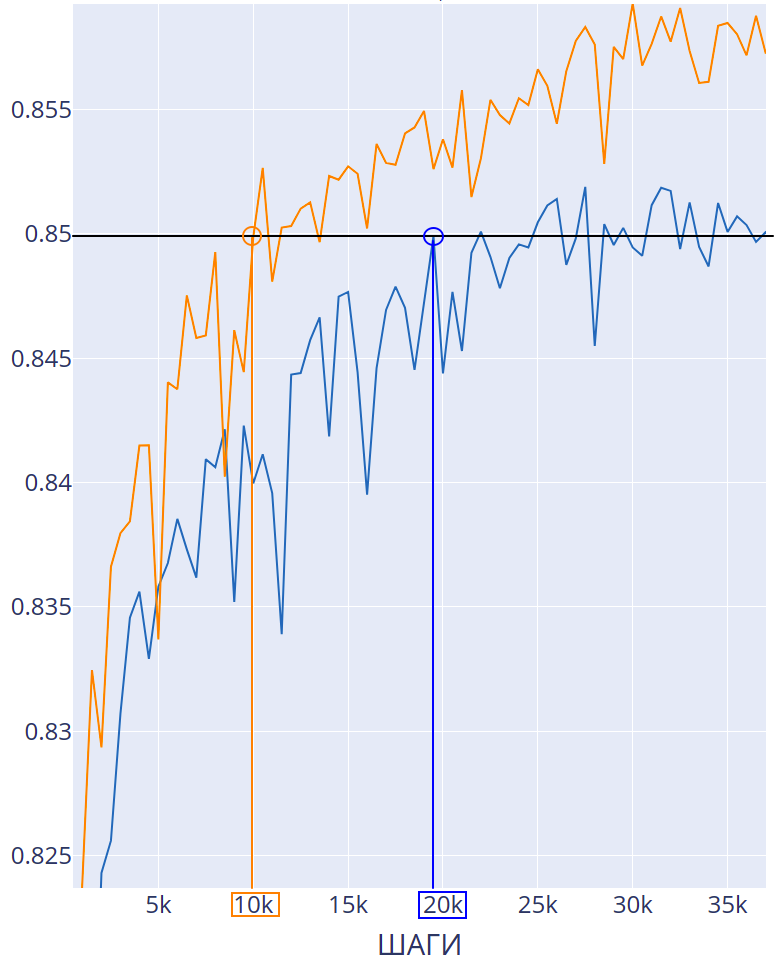
\includegraphics[scale=0.4]{compare}
	\caption{Среднее число шагов, необходимое для достижения порога $\alpha = 0.85$, $a_1 = 10k$, $a_2 = 20k$. Метод, соответствующий оранжевому графику, является лучшим.}
	\label{fig:metrics_compare}
\end{figure}

\subsection{Семплеры}
({\bf ОПИСАТЬ СЕМПЛЕРЫ})
\pagebreak
\subsection{Влияние обучения по плану на задаче предобучения}
\ 

\begin{figure}[h]
	\centering
	\begin{subfigure}{.3\textwidth}
		\centering
		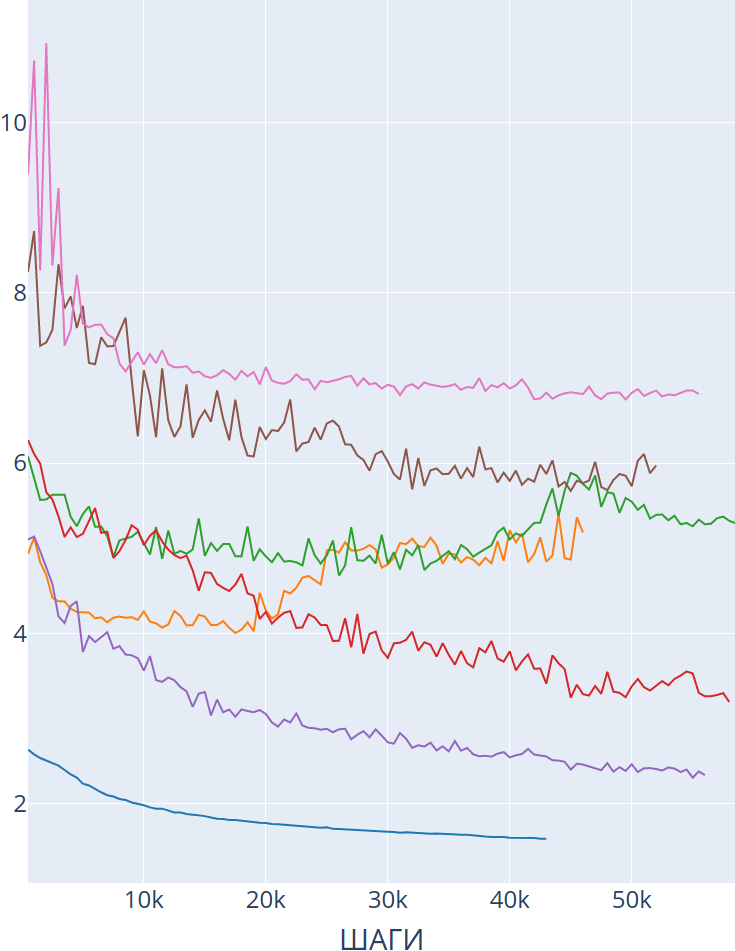
\includegraphics[scale=0.2]{BooksCorpus_CB}
		\caption{CB}
		\label{fig:BooksCorpus_graphs_CB}
	\end{subfigure}
	\begin{subfigure}{.3\textwidth}
		\centering
		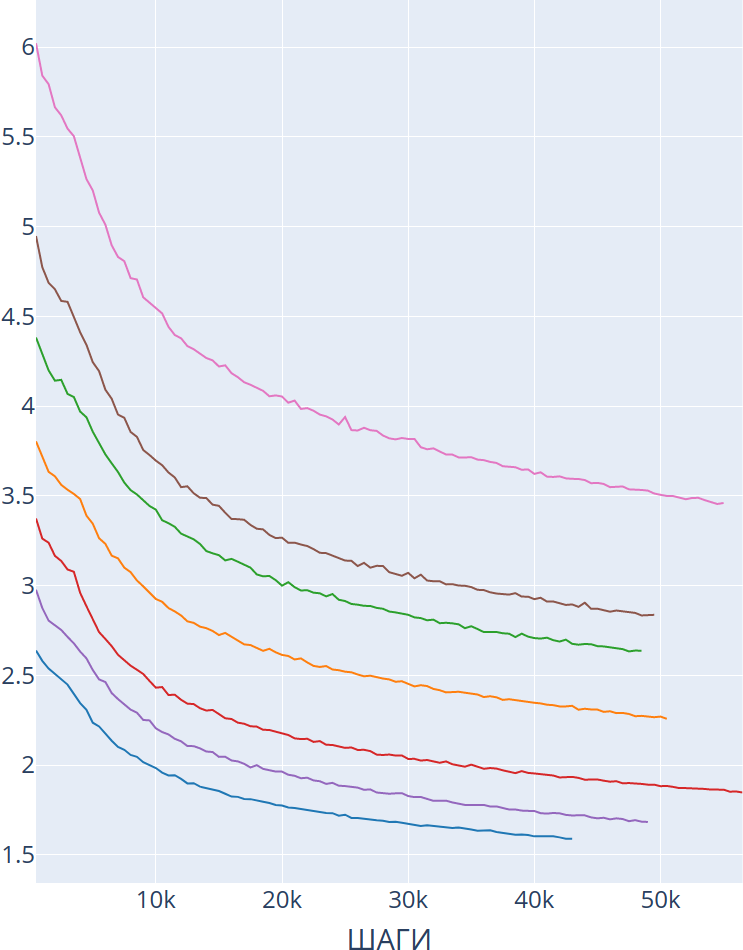
\includegraphics[scale=0.2]{BooksCorpus_DB}
		\caption{DB}
		\label{fig:BooksCorpus_graphs_DB}
	\end{subfigure}
	\begin{subfigure}{.3\textwidth}
		\centering
		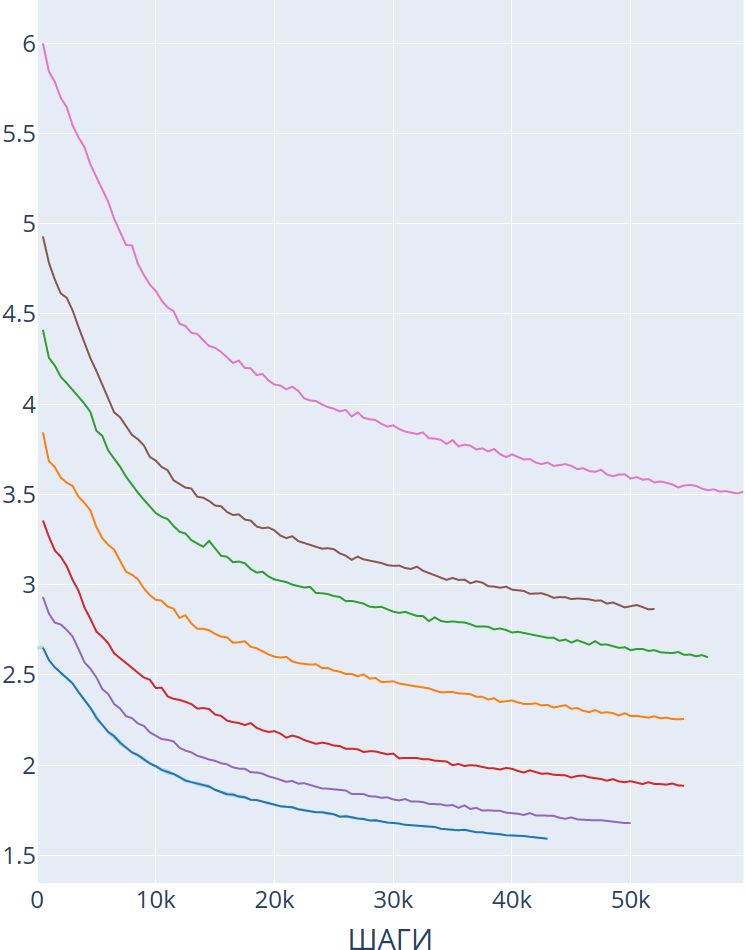
\includegraphics[scale=0.2]{BooksCorpus_Hyp}
		\caption{Hyp}
		\label{fig:BooksCorpus_graphs_Hyp}
	\end{subfigure}\\
	\begin{subfigure}{.3\textwidth}
		\centering
		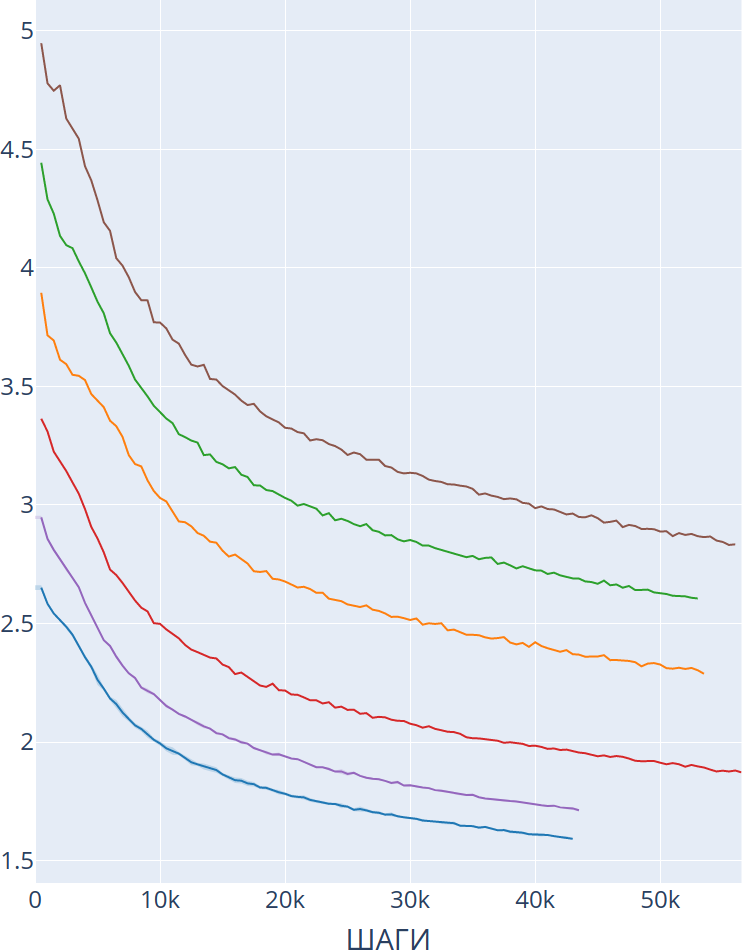
\includegraphics[scale=0.2]{BooksCorpus_SS}
		\caption{SS}
		\label{fig:BooksCorpus_graphs_SS}
	\end{subfigure}
	\begin{subfigure}{.3\textwidth}
		\centering
		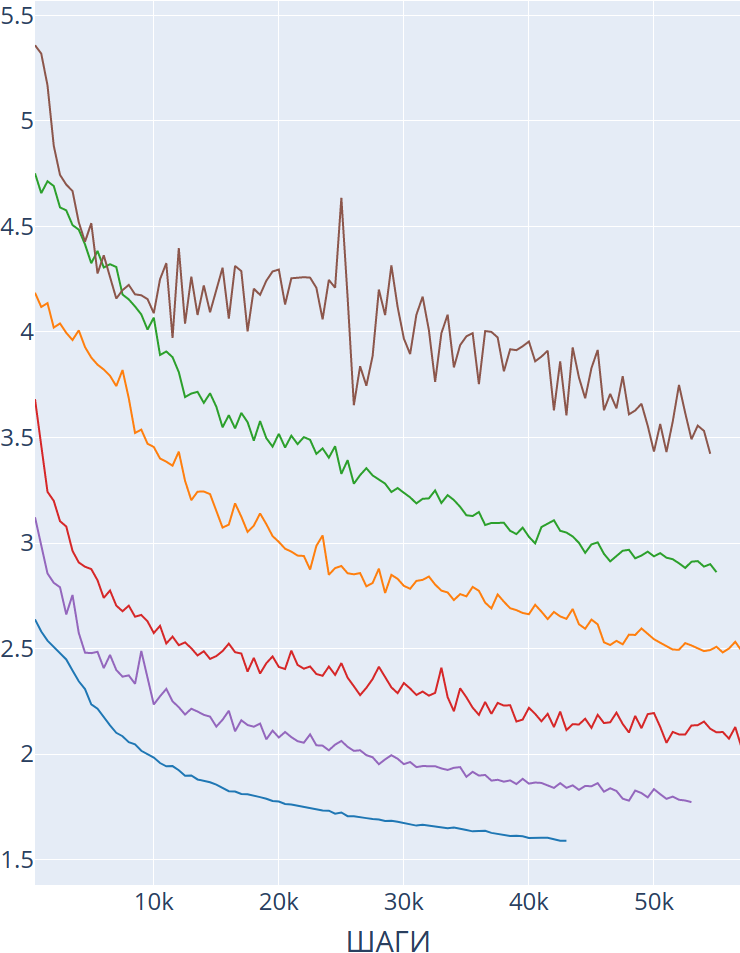
\includegraphics[scale=0.2]{BooksCorpus_SM}
		\caption{SM}
		\label{fig:BooksCorpus_graphs_SM}
	\end{subfigure}
	\begin{subfigure}{.3\textwidth}
		\centering
		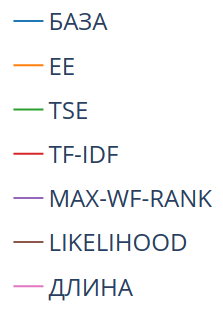
\includegraphics[scale=0.5]{BooksCorpus_legend}
		%		\caption{legend}
		\label{fig:BooksCorpus_graphs_legend}
	\end{subfigure}
	\caption{Графики зависимости функции потерь от числа шагов обучения на задаче предобучения на датасете BooksCorpus на первых 15\% обучения}
	\label{fig:BooksCorpus_graphs}
\end{figure}

\begin{table}
	\caption{Среднее число шагов всех конфигураций метрика-семплер на задаче предобучения на датасете BooksCorpus, необходимое для достижения порога. Максимальное стандартное отклонение $\Delta \le 3k$}.		\label{table:BooksCorpus_pretraining}
	\centering
	\begin{tabular}{|l|c|ccccc|c|}
		\hline
		Метрика & Порог & & \multicolumn{3}{c}{Семплеры} & & min loss\\
		\hline
		& & CB & DB & Hyp & SS & SM & \\
		\hline
		max wf rk & 2.00 & $\infty$ & 17.5k & {\bf 16.5k} & {\bf 16.5k} & 27k & {\bf 1.58} \\
		TF-IDF & 2.00 & $\infty$ & 34k & 35k & 37.5k & $\infty$ & 1.84 \\
		\hline
		\hline
		EE & 3.50 & $\infty$ & 4k & 3.5k & 4.5k & 9.5k & 2.25 \\
		TSE & 3.50 & $\infty$ & 9k & 9k & 8.5k & 18k & 2.60 \\
		правдоподобие & 3.50 & $\infty$ & 13.5k & 13.5k & 15.5k & 50k & 2.83 \\
		длина & 3.50 & $\infty$ & 50.5k & $\infty$ & - & - & 3.45 \\
		\hline
		\hline
		база & 2.00 & \multicolumn{5}{c}{9.5k} & 1.58 \\
		\hline
	\end{tabular}
\end{table}

Для исследования влияния обучения по плану на скорость обучения языковых моделей на задаче предобучения были проведены эксперименты с использованием всех конфигураций семплер-метрика за исключением метрики MLM\_loss, так как ее применение неразумно из-за того, что итогвоое время обучения возрастет как миниум в два раза: для вычисления метрики MLM\_loss нужна предобученная модель, а в рамках данной группы экспериментов такими моделями мы не располагаем. В итоге было получено $7\times 5$ графиков, которые можно наблюдать на рис. \ref{fig:BooksCorpus_graphs}. Можно заметить, что при использовании 4/5 семплеров метрики  образуют строгий порядок, а именно: максимальный ранг слова, TF-IDF, EE, TSE, вероятность правдоподобия и длина. На этих графиках виден сильный проигрыш обучения по плану по сравнению со стандартным алгоритмом обучения языковых моделей. Чтобы точнее определить разницу обратимся к таблице \ref{table:BooksCorpus_pretraining}. Во-первых, метрики разделены на две группы. Первая группа состоит из максимального ранга слова, TF-IDF. Вторая группа состоит из EE, TSE, вероятности правдоподобия и длины. Это связано с тем, что в первой группе метрики сходятся к гораздо более низким значениям по сравнению с метрками из второй группы. Следовательно тяжело выбрать такой порог, на котором можно было бы различать метрики внутри каждой группы. Таким образом можно сказать, что метрики из первой группы быстрее метрик из второй группы. Заметим, что в первой группе максимальный ранг слова позволяет получить такое же качество итоговой модели, как у базового подхода. В то время как остальные подходы такой возможности не предоставляют. К сожалению, приходится констатировать тот факт, что обучение по плану не ускоряет обучение моделей на задаче предобучения. Более того, применение обучения по плану приводит к замедлению от 2 до 5 раз.

\pagebreak
\subsection{Влияние обучения по плану на задаче классификации}

\begin{table}[h]
	\caption{Среднее число шагов всех конфигураций метрика-семплер на задаче классификации на датасете sentiment140, необходимое для достижения порога. Максимальное стандартное отклонение $\Delta \le 3k$}.
	\label{table:s140_fine_tuning}
	\centering
	\begin{tabular}{|l|c|ccccc|c|}
		\hline
		Метрика & Порог & & \multicolumn{3}{c}{Семплеры} & & Точность\\
		\hline
		& & CB & DB & Hyp & SS & SM &\\
		\hline
		длина & 85.5\% & 112.5k & 20k & 19k & - & - & {\bf 86.2\%} \\
		{\bf TF-IDF} & 85.5\% & 115.5k & 21.5k & 19.5k & {\bf 16.5k} & 22k & 86.7\% \\
		{\bf TSE} & 85.5\% & 95.5k & {\bf 16.5k} & 20.5k & 21.5k & 18k & 86.8\% \\
		EE & 85.5\% & 59k & 19.3k & 23k & 20k & 19k & 86.7\% \\
		{\bf max wf rk} & 85.5\% & 70k & 18.5k & 19.5k & {\bf 17k} & 19k & 86.7\% \\
		правдоподобие & 85.5\% & 112k & 17.5k & 21.5k & 17.5k & 21.5k & 86.7\% \\
		MLM-loss & 85.5\% & 59.5k & 21k & 23.5k & 19.5k & 20k & {\bf 86.1\%} \\
		\hline
		база & 85.5\% & & \multicolumn{3}{c}{17.5k} & & 87\% \\
		\hline
	\end{tabular}
\end{table}

\begin{table}[h]
	\caption{Среднее число шагов всех конфигураций метрика-семплер на задаче классификации на датасете Hyperpartisan News Detection, необходимое для достижения порога. Максимальное стандартное отклонение $\Delta \le 3k$}.
	\label{table:hnd_fine_tuning}
	\centering
	\begin{tabular}{|l|c|ccccc|c|}
		\hline
		Метрика & Порог & & \multicolumn{3}{c}{Семплеры} & & Точность\\
		\hline
		& & CB & DB & Hyp & SS & SM & \\
		\hline
		длина & 92.9\% & 55k & 23k & 22.5k & - & - & 93.7\% \\
		TF-IDF & 92.9\%  & $\infty$ & {\bf 19.5k} & 24k & 23.5k & 33k & 93.5\% \\
		TSE & 92.9\% & 56.5k & {\bf 21k} & 23k & 22k & 31k & 93.8\% \\
		EE & 92.9\%  & 71.5k & 25.5k & 22.5k & {\bf 19.5k} & 32.5k & 93.8\% \\
		max wf rk & 92.9\%  & $\infty$ & 22k & {\bf 20.5k} & 22.5k & 39k & 93.6\% \\
		правдоподобие & 92.9\% & $\infty$ & {\bf 20k} & 24k & {\bf 20k} & 30k & 93.8\% \\
		MLM-loss & 92.9\% & 23.5k & {\bf 18k} & 23k & 24k & 20k & {\bf 93.9\%} \\
		\hline
		база & 92.9\%  & \multicolumn{5}{c}{22k} & 93.8\% \\
		\hline
	\end{tabular}
\end{table}

Перейдем к описанию результатов применения обучения по плану на задаче классификации. Здесь были произведены эксперименты со всеми метриками на двух корпусах данных: sentiment140 и Hyperpartisan News Detection. Обратимся к таблицам \ref{table:s140_fine_tuning} и \ref{table:hnd_fine_tuning}. Во-первых, заметим, что на датасете sentiment140 при использовании обучения по плану проседает итоговая точность модели на 0.3\% для всех метрик кроме длины и MLM\_loss (на них просадка в 0.8\% и 0.9\% соответственно), в то время как на датасете Hyperpartisan News Detection этого не происходит. Возможная причина заключается в том, что sentiment140 содержит тексты меньшей длины, следовательно для выразительной модели BERT сложность примеров почти неразличима. Однако, это утверждение ложно до определенного момента. Если выбрать высокий порог точности в 85.5\% (-1.5\% итоговой точности), то разница в метриках существенна, а именно метрики TF-IDF, TSE и максимальный ранг слова приводят к хоть и не значительному, но ускорению обучения на 3\%. Остальные метрики замедляют скорость сходимости модели. Также заметим, что при увеличении размера датасета (sentiment140 $\rightarrow$ HND) в множество ускоряющих метрик $\{\text{TF-IDF, max-wf rk, TSE}\}$ добавляются остальные. Это соотносится с экспериментами на задаче предобучения. Там наиболее быстрыми метриками являлись максимальный ранг слова и TSE. Длина же ни в одной конфигурации не позволяет ускорить обучение модели, что подтверждает гипотезу о том, что данная метрика не является разумным выбором метода оценки сложности текстов в контексте обучения по плану. Еще один важный вывод заключается в том, что модель не всегда может выдать правильную характеристику примеру относительно его сложности (MLM\_loss не ускоряет обучение модели и ухудшает итоговое качество на датасете sentiment140)). Это происходит тогда, когда модель достаточно выразительна и для нее все примеры имеют одинаковую сложность с точки зрения модельной метрики. В этом можно убедиться, если посмотреть на результаты на датасете HND из более длинных примеров. На нем метрика MLM-loss увеличивает качество итоговой модели на 0.1\% и ускоряет обучение с 22k до 18k шагов.

\pagebreak
\subsection{Влияние обучения по плану на шумном корпусе данных}
\ 

Важным случаем в машинном обучении является ситуация, когда приходится обучать модели на шумных наборах данных. Такое может встречаться у компаний, которые автоматически собирают данные. Например, можно построить корпус данных, основываясь на открытых сообщениях некоторого форума. Очевидно, люди при использовании подобных сервисов не уделяют должного внимания грамотности и пунктуации написанных сообщений. Для их очистки требуются существенные денежные ресурсы. Также, данный случай рассматривается в аналогичных работах, изучающих влияние обучения по плану на скорость сходимости моделей. Например, Wu и его коллеги в работе \cite{wu2020curricula} показали, что обучение по плану негативно влияет на качество итоговой модели и скорость обучения на задаче классификации картинок. Однако, они нашли полезное применение данной техники в случае обучения на шумном корпусе данных. Важно отметить, что шум оказывает довольно сильное влияние на большие языковые модели. В этом можно убедиться, если обратиться к работе \cite{srivastava2020noisy}. Поэтому важной задачей является быстрое и качественное обучение моделей в подобных окружениях. В данном блоке экспериментов будет исследовано влияние обучения по плану на скорость сходимости языковой модели BERT при ее обучении на шумном наборе данных.

Для эмуляции описанной выше ситуации мы искусственно добавим шум в корпус данных. В работе~\cite{srivastava2020noisy}, в которой исследуется влияние шума на языковую модель BERT, авторы предложили так называемый клавиатурный шум. Чтобы его применить к тексту, нужно взять какую-то долю символов и заменить их на случайного соседа на стандартной QWERTY клавиатуре. Помимо этого шума в данной работе предложено рассмотреть еще два вида шумов: ошибки произношения и случайные перестановки нескольких символов в слове. Алгоритм зашумления текстовых данных выглядит следующим образом.

\begin{enumerate}
	\item Выбираем случайное число $\rho \sim U[0, \rho_{max}]$
	\item Применяем шум с долей испорченных символов равной $\rho$
\end{enumerate}

Сначала необходимо проверить, помогает ли в целом обучение по плану в данной конфигурации. Заметим, что при добавлении шума мы работали с величиной $\rho$, которая является уровнем шума. Выяснилось, что если взять $\rho$ в качестве метрики оценки сложности текстов, то это позволяет значительно ускорить обучение модели в самом начале тренировки (см. рис. \ref{fig:s140_noise_lvl}). Однако, в реальности мы не обладаем никаким знанием о том, сколько шума находится в конкретном примере, поэтому нужно придумать метрику, которую можно вычислить, не опираясь на знания о шуме. Вторым критерием служит сильная корреляция данной метрики с уровнем шума. Наблюдения за данными показали, что в шумных примерах среднее число токенов на слово сильно больше, чем в чистых. Это связано с устройством токенизаторов, в словарях которых большинству токенов соответствуют наиболее частые слова в языке. При добавлении шума предложение содержит большое количество слов, которых нет в словаре. Следовтаельно, токенизатору приходится разбивать слово на несколько частей и описывать каждую из них отдельным токеном.
	
Эксперименты показали, что шумы ведут себя одинаково в контексте обучения по плану, поэтому далее я буду описывать результаты с использованием клавиатурного шума. Выяснилось, что все метрики, кроме TPW, замедляют обучение. Использование метрики TPW вместе с лестничным семплером из четырех ступенек приводит к тому, что модель обучается до 95\% итоговой точности (например, 83\% из 87\%) в два раза быстрее по сравнению с обучением без плана (см. рис. \ref{fig:s140_noise_tpw}). Данное явление можно описать следующим образом. Как показывает таблица \ref{table:tokenize_noisy_text} использование метрики TPW в обучении по плану приводит к тому, что модель вначале своей тренировки обучается на чистых примерах, плавно переходя к более шумным, что приводит к стаблильной тренировке и позволяет намного быстрее добиться существенного качества. Важно отметить, что описанный подход можно применять на практике, а именно если у компании стоит задача в кратчайшие сроки получить некоторый прототип работающего приложения, но на момент постановки задачи не имеется очищенного датасета.

\begin{figure}[h]
	\centering
	\begin{subfigure}{.45\textwidth}
		\centering
		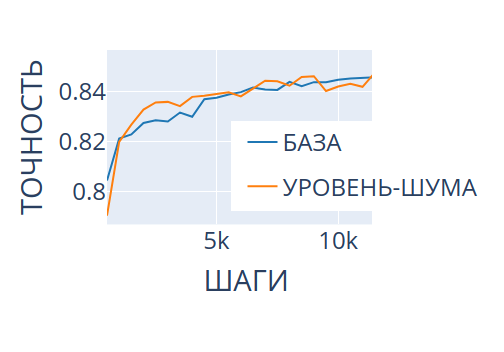
\includegraphics[scale=0.5]{keyboard_noise_level_short_prefix}
		\caption{Метрика "уровень шума"}
		\label{fig:s140_noise_lvl}
	\end{subfigure}
	\begin{subfigure}{.45\textwidth}
		\centering
		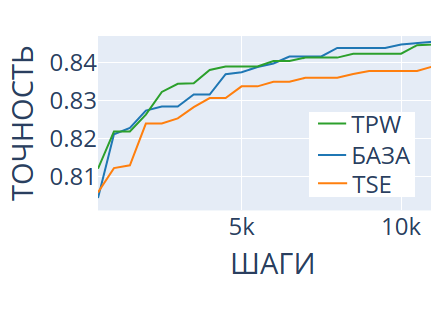
\includegraphics[scale=0.5]{keyboard_noise_TPW_win}
		\caption{Метрика TPW}
		\label{fig:s140_noise_tpw}
	\end{subfigure}
	\caption{Графики зависимости точности от числа шагов обучения на задаче классификации на датасете sentiment140 для достижения 95\% итоговой точности при добавлении клавиатурного шума}
	\label{fig:s140_noise}
\end{figure}

\pagebreak
\subsection{Выводы}
\ 

В данной главе была описана экспериментальная часть работы. Мною были сформулированы конфигурации экспериментов и описаны их результаты. В ходе исследований выяснилось, что:

\begin{enumerate}
	\item Обучение по плану замедляет скорость обучения от 2 до 5 раз на задаче предобучения языковых моделей
	\item Обучение по плану не позволяет существенно ускорить обучение на задаче классификации текстов, однако существует узкий (TSE+DB на sentiment140, MLM-loss+DB на HND) набор конфигураций, который приводит к ускорению на 3\% в среднем в сравнении с обучением без плана
	\item Найден частный случай (классификация текстов с добавлением шума), на котором применение обучения по плану приводит к ускорению обучения в два раза для достижения 95\% итоговой точности модели, и метрика (TPW) для достижения этого результата
\end{enumerate}

\section*{Заключение}
\ 

В результате проделанной исследовательской работы выяснилось, что существует сильно ограниченный набор конфигураций, в рамках которых обучение по плану позволяет ускорить обучение. Данное множество настроек было найдено за счет расширения набора метрик оценки сложности текстовых данных. На задаче предобучения языковых моделей лучшая метрика "максимальный ранг слова" замедляет обучение модели от 2 до 5 раз. На задаче классификации текстов метрики TF-IDF, TSE и "максимальный ранг слова" позволяют сократить число тренировочных шагов на 3\% в среднем. Рассмотрение важного частного случая обучения моделей на шумных тренировочных данных позволило выявить метрику TPW, которая позволяет обучать модели до 95\% итоговой точности в два раза быстрее по сравнению с обучением без плана. Описанные результаты лишний раз подчеркивают тот факт, что обучение по плану невозможно применить к любой задаче без тонкого подбора параметров и без правильного выбора метрики. Таким образом, было исследовано влияние обучения по плану на задаче предобучения языковых моделей и классификации текстов на скорость схоимости моделей, расширено множество рассматриваемых метрик оценки сложности текстов и исследован важный частный случай применения обучения по плану на задаче классификации текстов при условии наличия лишь шумных тренировочных данных.

Исследования в данной области можно продолжать в следующих направлениях:

\begin{itemize}
	\item Направление 1
	\item Направление 2
	\item Направление 3
	\item Направление 4
\end{itemize}

% размещенный с предпочтением "вверху страницы"
% \begin{figure}[t]
% \centering
% 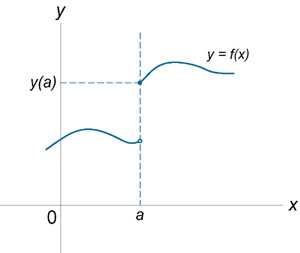
\includegraphics{fig1.jpg}
% \caption{Разрыв функции}
% \label{разрыв_функции}
% \end{figure}

% [h]
    % 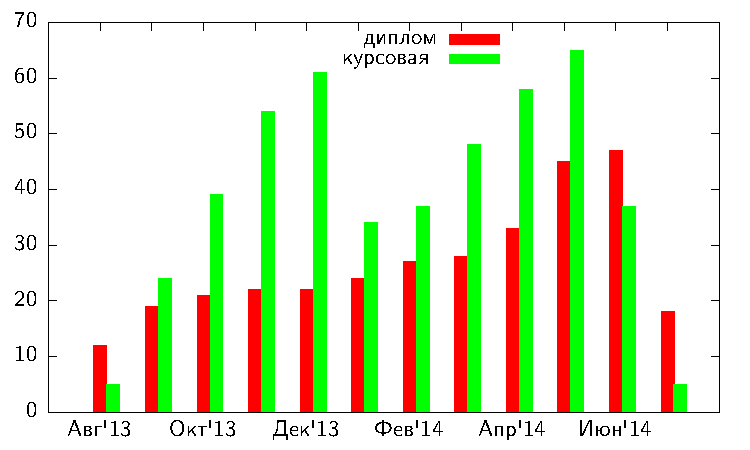
\includegraphics{thesis-search-trends}
    % \caption{Статистика поисковых запросов в течении года}
% \end{figur

\bibliographystyle{ugost2008ls}
\bibliography{diploma.bib}
\end{document}
